\chapter{Introduction}
\label{cha:introduction}

The recent development in the deep learning area has resulted in a significant increase in usage of artificial intelligence
solutions. Recommendation algorithms, voice or face recognition, type hinting - these are only examples of technologies which are
used on everyday basis by millions. Deep Artificial Neural Networks are by far the most robust of all machine learning
algorithms capable of handling various tasks in an unprecedented manner. Thus the choice of getting hands on designing and
implementing vision system for an autonomous boat which uses their full potential.

\section{Purpose and structure}
\label{sec:purpose}

The goal of the Thesis was to create a \textbf{vision system} for an autonomous agent which would be responsible for its autonomous control
on a given track limited by buoys. The system uses images retrieved from a pair of front cameras to train a \textbf{Deep Reinforcement
Network} responsible for track analysis and boat control. The entire project is held in a simulation environment where a designed algorithm
is trained on a boat model which resembles a real life counterpart. 

The expected result was a well-designed and trained Deep Reinforcement Network capable of controlling the boat within defined constraints.
Ideally the network should be tested in a real environment, however due to limited resources and time the overall performance was measured
entirely in the simulation.

This chapter contains a brief overview of Reinforcement Learning applications. The next three chapters introduce mathematical basis and
explanation of underlying concepts of Deep Learning, Convolutional Neural Network and Reinforcement Learning respectively. The fifth
chapter describes the Vision System project followed by research results and conclusion in chapters \ref{cha:results} and \ref{cha:conclusion}.

\newpage

\section{Real-life applications of Reinforcement Learning}
\label{sec:real-life-applications-of-deep-learning}

\subsection{Games}
\label{sub:intro-games}
Reinforcement Learning nowadays is well-known due to algorithm which used to play different games and managed to achieve a super-human performance in some.
The Deep Q-Network agent designed by \emph{Google Deep Mind} was able to play 49 different Atari 2600 games (figure \ref{fig:Atari2600}). However, the most
famous one is probably the \emph{AlphaGo} \cite{AlphaGO}  and \emph{AlphaGo Zero}. AlphaGo was trained on countless human games achieving
robust performance, but it was not sufficient for the researchers. They let their new agent trained from scratch - AlphaGo Zero to play with
itself and eventually beat AlphaGo 100-0. 

\begin{figure}[h]
    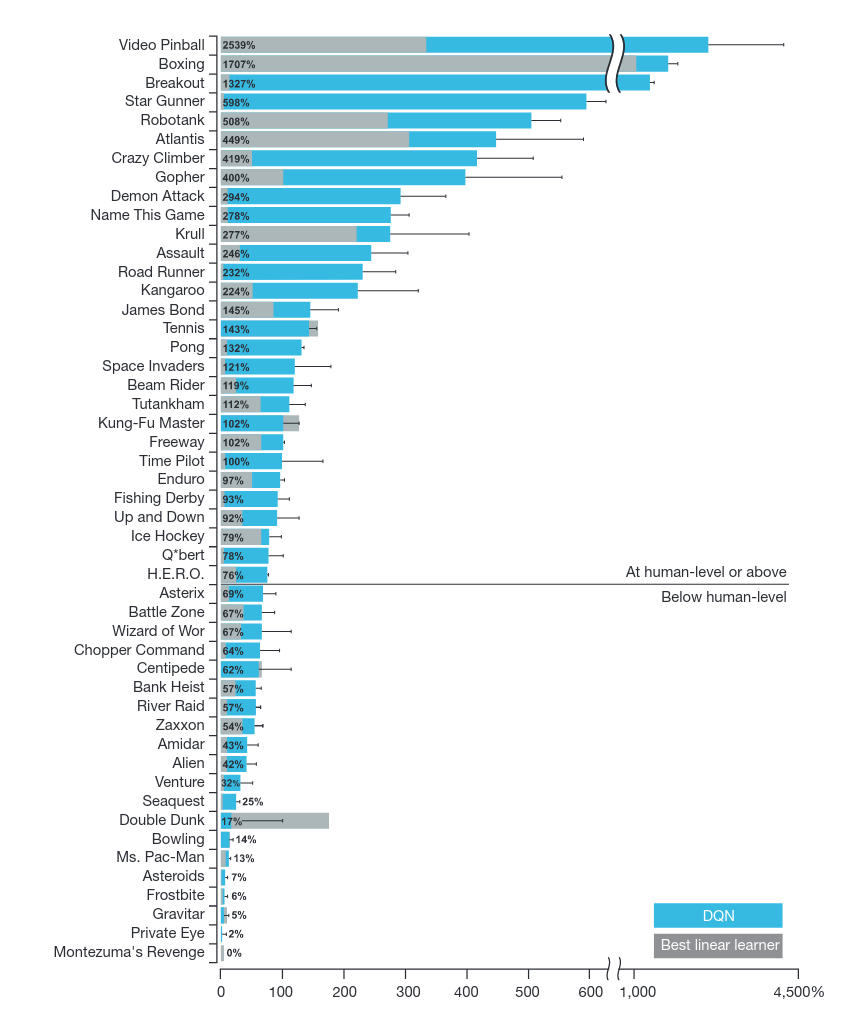
\includegraphics[width=12cm]{img/Atari2600.png}
    \centering
    \caption{Reinforcement Learning model vs human-level performance in the Atari 2600 environment \cite{DQNAtari}.}
    \label{fig:Atari2600}
\end{figure}

\subsection{Robotics}
\label{sub:intro-robotics}
As stated in survey conducted by \emph{Jens Kober}, \emph{J.Andrew Bagnell}, and \emph{Jan Peters} \cite{RNSurvey}, ``\emph{Reinforcement
learning offers to a robotics a framework and set of tools for the design of sophisticated and hard-to-engineer behaviors}''. In fact, these
are most of existing ones in a real world. Instead of engineering a set of deterministic movements of a robot in a controlled environment,
identical or improved result can be achieved through training in a well-defined task which provides feedback measuring robot's performance.
Such approach enables to train robots for performing tasks in more real world environments which are not usually fully controllable.

\subsection{Personalized Recommendations}
\label{sub:intro-personalized-reccomendations}
News recommendations tends to be challenging due to the fact that most of the users easily get bored. Even if one clicks at the article,
there is a low likelihood that it will be read to the end. Therefore Click Through Rate standalone, which is used by many algorithms, is an
ineffective indicator. In order to improve the quality of recommendations and address this issue, the DQN was designed and described in
\emph{DRN: A Deep Reinforcement Learning Framework for News Recommendation} \cite{DRNNewsRecommendaiton}. This method uses multiple features
to determine what will be displayed to the user.
